\documentclass{fkssolpub}

\usepackage[czech]{babel}
\usepackage{fontspec}
\usepackage{fkssugar}
\usepackage{amsmath}
\usepackage{graphicx}

\author{Ondřej Sedláček}
\school{Gymnázium Oty Pavla} 
\series{74-I}
\problem{6} 

\begin{document}

\begin{figure}
	\begin{center}
		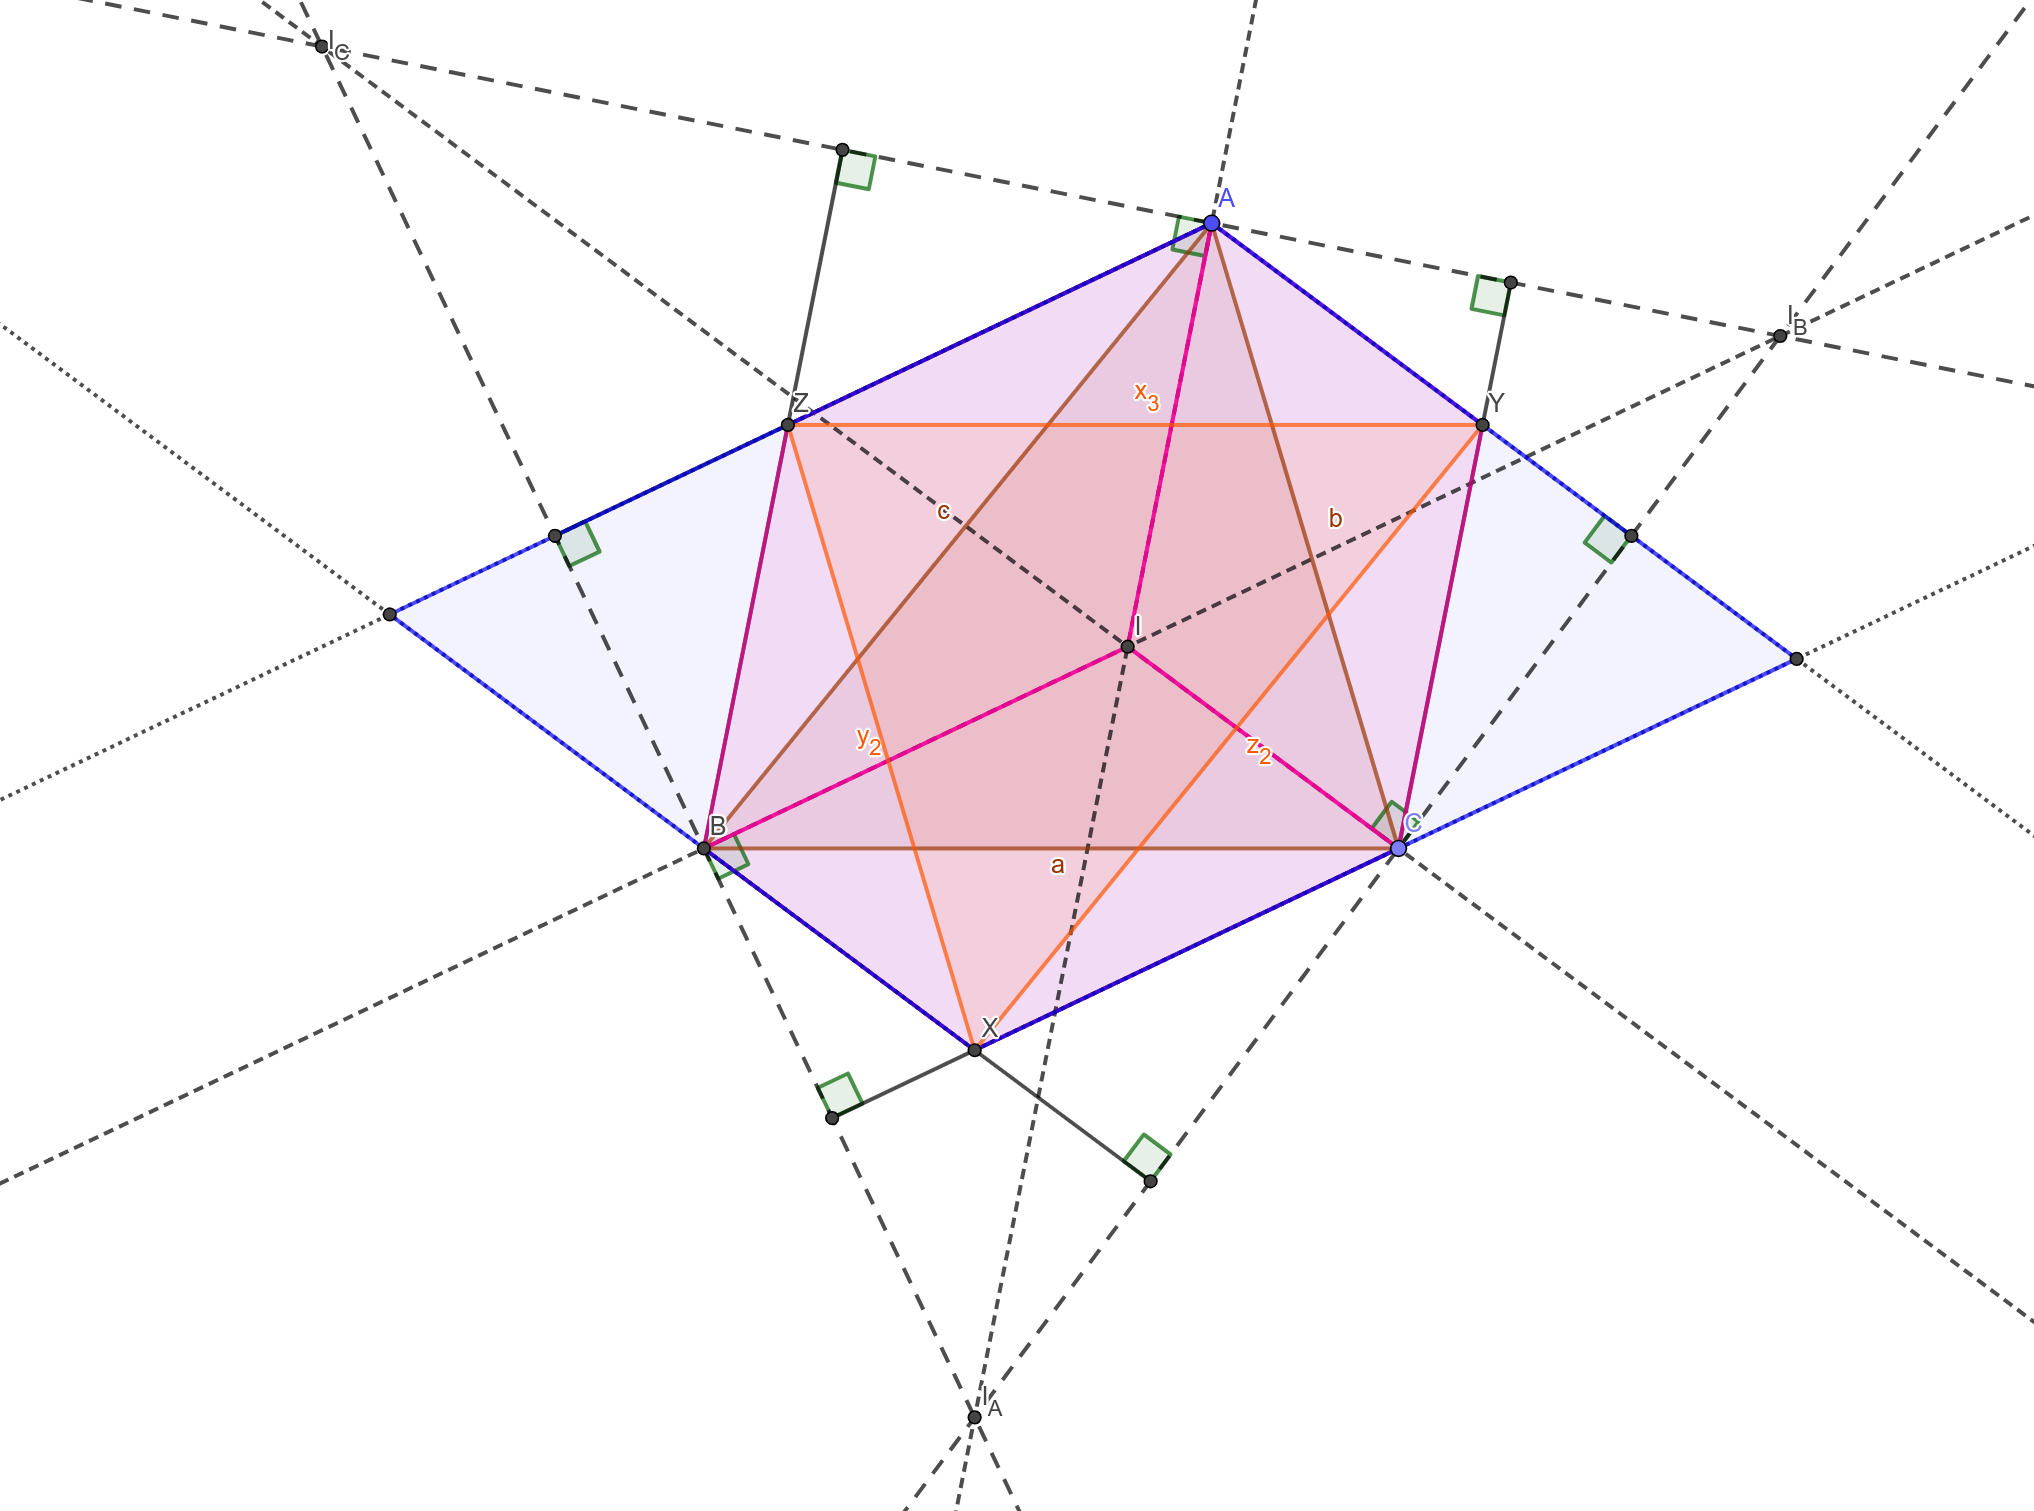
\includegraphics[width=0.95\textwidth]{6-fig.png}
	\end{center}
	\caption{Konstrukce úlohy}
	\label{fig:1}
\end{figure}

Jako první si musíme uvědomit, že osa vnitřního úhlu a osa vnějšího úhlu při určitém vrcholu jsou si kolmé, protože $\frac{\alpha}{2} + \frac{180 - \alpha}{2} = \frac{180}{2} = 90^{\circ}$. Z toho víme, že $BZ \parallel AI \parallel CY$, $AZ \parallel BI \parallel CX$ a $AY \parallel CI \parallel BX$, protože tyto výšky jsou také kolmé na osu vnějšího úhlu. Z těchto rovnoběžností tedy nutně platí, že čtyřúhelníky $BIAZ$, $ICYA$ a $XCIB$ jsou rovnoběžníky, z čehož nutně platí, že $|BZ| = |AI| = |CY|$, $|AZ| = |BI| = |CX|$ a $|AY| = |CI| = |BX|$.

Teď už nám zbývá ukázat, že protější úhly v šestiúhelníku $AZBXCY$ jsou stejně velké. Když prodloužíme ramena těchto úhlů, vznikne nám v rovině rovnoběžník, protože protější strany tohoto šestiúhelníku jsou rovnoběžné. A poněvadž tyto protější úhly musí být nutně protější i v tomto rovnoběžníku, musí být protější úhly v tomto šestiúhelníku stejně velké.

S tím vším už umíme najít shodné trojúhelníky $AZY \cong XCB$, $YAC \cong BXZ$ a $ZAB \cong CYX$ pomocí věty sus. Z těchto trojúhelníků nutně platí, že $|AB| = |XY|$, $|BC| = |YZ|$ a $|CA| = |ZX|$, tedy podle věty sss jsou trojúhelníky $ABC$ a $XYZ$ shodné. Tím je tedy důkaz u konce.

\end{document}
